
\chapter{CONTROLLERS}
\label{chap:Controllers}

The control requirements for NASA MMS TableSat 1A can be simplified into three main goals.

First is to maintain a steady spin rate of 3 rpm ($\pi/10$ rad/sec).  Given the relative success of the body rate estimation in Section \ref{chap:Estimators}, this goal should be attainable without the need of advanced control efforts.

Second is to correct for any nutation detected by the estimator.  This requirement can take the form of both driving body rates $\omega_y$ and $\omega_z$ to zero, and ensuring the estimated quaternion's Euler axis is kept in line with the global reference frame's $z$-axis.

Third is to prevent and/or remove oscillations in the Axial Double Probe (ADP) and Spin-plane Double Probe (SDP) booms.  Out of the three, this performance goal has the largest set of dependencies for success.  This level of control is reliant on effective actuators along with reliable state estimates based on an accurate system model which include boom dynamics.

The first two goals is addressed in this chapter as their scope is limited to controller design.  Section \ref{sec:ActuatorConfiguration} covers the configuration of the actuators on TableSat and how their configuration is incorporated into the controller code.  The remaining sections of this chapter focus on the rate and nutation control methods, and use the assumption that the estimators are providing perfect state measurements.  This temporarily limits the scope of the testing to ensure that the control techniques are being implemented properly in the software especially since with the development of some non-standard techniques.  The boom oscillations control goal is addressed in Chapter \ref{chap:ObserverBasedControls} when multiple modules are be linked together to get a wider view of the interactions between sections of observer-based controller acting on noisy state measurements.

\section{Actuator Configuration}
\label{sec:ActuatorConfiguration}

The actuators in use on NASA MMS TableSat 1A consists of four single directional computer fans.  Two oriented for rate control and two for nutation control.  The body rate control fans are mounted on opposite sides of the deck with their thrusts applying opposing moments.  The two nutation fans are mounted flush with the deck at a 90 degree offset and have their thrust directed down.  The fans are assumed to be mounted such that the moments are applied about orthogonal axes.  This simplifies the actuator module's voltage calculations for each fan which can be improved if testing shows the effects are significant enough to compensate for.  Four analog ports to the Athena PC are available for actuator usage after mounting the sensors.  Two dedicated to the rotational fans to provide full rotational control, and the remaining two provide partial nutation control.
\begin{figure}[H]
  \centerline{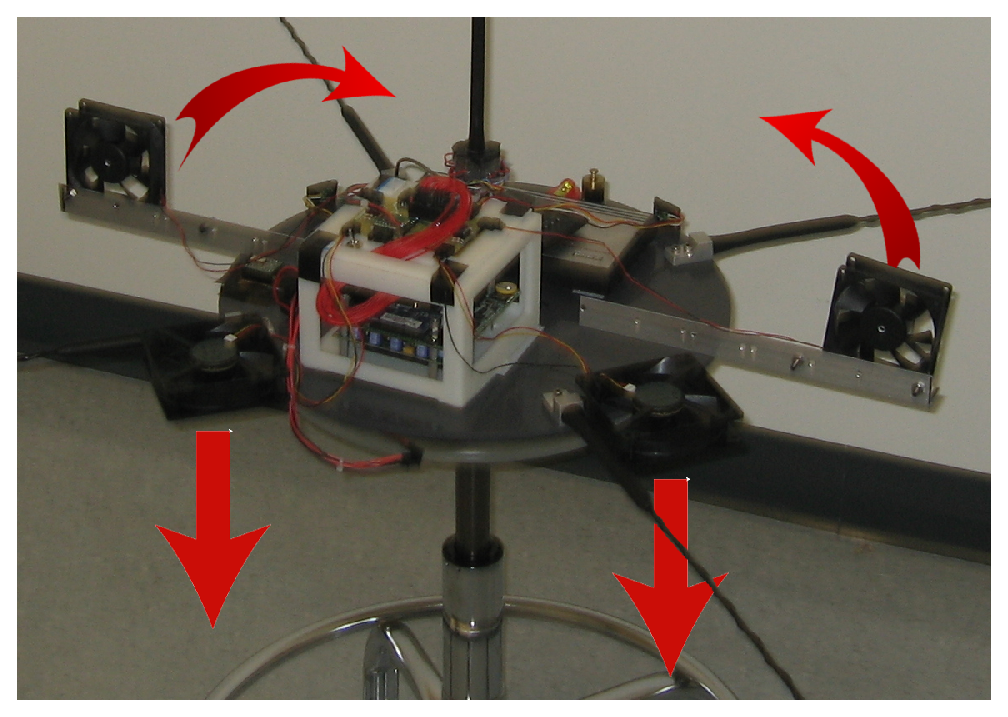
\psfig{file=figures/tsat_thrusters.eps,height=3in}}
  \caption{NASA MMS TableSat 1A thrusters}
  \label{fig:TSatThrusters}
\end{figure}
Passing the desired moments from the controller directly to the estimator without taking the fan geometry into consideration would create a disconnect between the estimated and actual system states.  The software's actuator module is designed to accept a list of fans with their center, direction of thrust related to the body reference frame, and maximum force to determine the moments couples that are actually possible.
\begin{figure}[H]
  \centerline{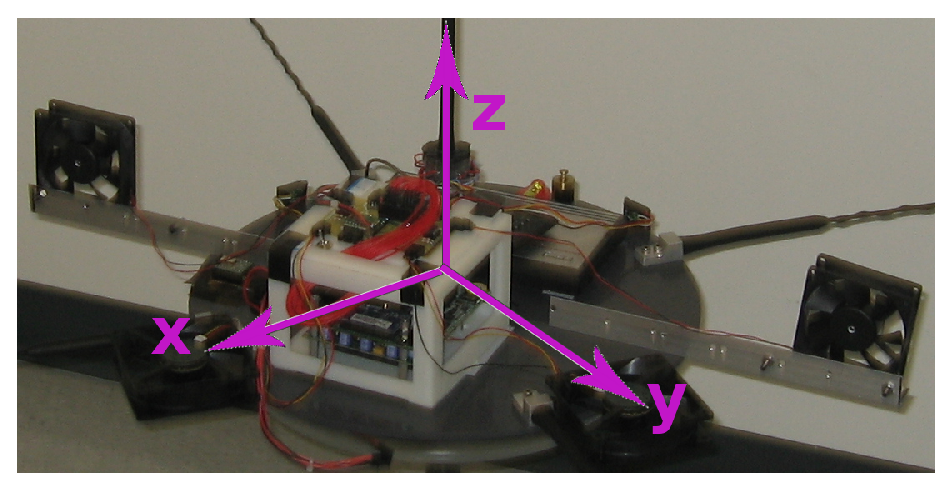
\psfig{file=figures/tsat_body_axes.eps,height=3in}}
  \caption{NASA MMS TableSat 1A Body Axes}
  \label{fig:TableSatBodyAxes}
\end{figure}
Table \ref{tbl:ActuatorConfiguration} shows the fan configuration for the NASA MMS TableSat 1A as arranged in Figure \ref{fig:TSatThrusters}.
\begin{table}[H]
  \centering
  \begin{tabular}{c|c|c|c|c}
    Fan & Center $\bs{f_c}$ (m) & Direction $\bs{n}$ & $F$ (N) & Max Moment $\frac{F \bs{n} \times \bs{f_c}}{|\bs{n}|}$ (Nm) \\ \hline
    1 & $(0.2474, -0.2474, 0)$ & $(-1, -1, 0)$ & 0.08 & $(0, 0, 0.039598)$ \\
    2 & $(-0.2474, 0.2474, 0)$ & $(-1, -1, 0)$ & 0.08 & $(0, 0, -0.039598)$ \\
    3 & $(0.25, 0, 0)$ & $(0, 0, -1)$ & 0.08 & $(0.02, 0, 0)$ \\
    4 & $(0, 0.25, 0)$ & $(0, 0, -1)$ & 0.08 & $(0, -0.02, 0)$ \\
  \end{tabular}
  \caption{Actuator configuration}
  \label{tbl:ActuatorConfiguration}
\end{table}
The code snippet below demonstrates the actuator module's functionality as it has been implemented in the TSatPy software.  Lines 4-13 define the geometry of the actuators displayed in Figure \ref{fig:TSatThrusters} with the addition of a hypothetical fifth actuator along with their center, direction of thrust, and maximum thrust force.

\begin{singlespace}
  \begin{minted}[mathescape,linenos,numbersep=10pt,frame=lines,framesep=2mm]{python}
import numpy as np
from TSatPy.Actuator import Actuator

configs = [{'type': 'fan', 'args': {'name': 'CW',
  'center': (0.2474, -0.2474, 0), 'direction': (-1, -1, 0), 'F': 0.08}
},{'type': 'fan', 'args': {'name': 'CCW1',
  'center': (-0.2474, 0.2474, 0), 'direction': (-1, -1, 0), 'F': 0.08}
},{'type': 'fan', 'args': {'name': 'CCW2',
  'center': (-0.2474, -0.2474, 0), 'direction': (1, -1, 0), 'F': 0.08}
},{'type': 'fan', 'args': {'name': 'NY', 'center': (0.25, 0, 0),
  'direction': (0, 0, 1), 'F': 0.08}
},{'type': 'fan', 'args': {'name': 'NX', 'center': (0, 0.25, 0),
  'direction': (0, 0, 1), 'F': 0.08}}]

def set_level(act, power_level):
    print 'Setting power level=%g for: %s' % (power_level, act)

def setup_actuators(configs):
    act = Actuator()
    for config in configs:
        act.add(config['type'], set_level, config['args'])
    return act

act = setup_actuators(configs)
print(act)
M = np.mat([0.03, 0.11, 0.04]).T
print("Request moment: %s" % (M.T))
print("Applied moment: %s" % (act.request_moment(M).T))

# Prints Out
# Actuator
#  <Fan CW moment=(0, -0, -0.0279901)>
#  <Fan CCW1 moment=(0, 0, 0.0279901)>
#  <Fan CCW2 moment=(0, 0, 0.0279901)>
#  <Fan NY moment=(0, -0.02, 0)>
#  <Fan NX moment=(0.02, 0, 0)>
# Request moment: [[ 0.03  0.11  0.04]]
# Setting power level=1 for: <Fan NX moment=(0.02, 0, 0)>
# Setting power level=0.714538 for: <Fan CCW1 moment=(0, 0, 0.0279901)>
# Setting power level=0.714538 for: <Fan CCW2 moment=(0, 0, 0.0279901)>
# Applied moment: [[ 0.02  0.    0.04]]
  \end{minted}
\nocite{minted}
\end{singlespace}

At line 24, the actuator instance is created and each fan's potential contribution to the overall control moment is calculated with
\begin{equation}
  \bs{M} = \frac{F \bs{n} \times \bs{f_c}}{|\bs{n}|}
\end{equation}
The script output shown above describes how a requested moment of $M_x = 0.03Nm, M_y = 0.11Nm, M_z = 0.04Nm$ would be applied to the five fan configuration.  The ``Nx'' fan can only produce a $0.02Nm$ moment, so gets set to full power to supply part of the requested $M_x = 0.03Nm$.  The ``Ny'' fan does not contribute since it's thrust is in the opposite direction from the needed $M_y = 0.11Nm$.  The ``CCW1'' and ``CCW2'' fans can not individually meet the requested $M_z = 0.04Nm$, but are able to collaboratively reach the requested moment by contributing 71\% each.  In the end, the actual moment that would be applied to the s/c is $M_x = 0.02Nm, M_y = 0Nm, M_z = 0.04Nm$.  This actual moment is both converted to voltages to be transmitted to the TableSat and supplied to the feedback loop to update the estimator's state propagation.

\section{Rate Control}
\label{sec:RateControl}

The first of the three controls goals introduced at the start of this chapter, is to attain a body rate of
\begin{equation}
  \bs{\omega}_d = 0 \bs{i} + 0 \bs{j} + 0.314 \bs{k}
\end{equation}
This desired rate is used for the tests in Sections \ref{subsec:PRateControl} through \ref{subsec:ComparativeAnalysisofPIDandSMCRateControl}.  As explained at the start of the chapter, the following iterations of body rate controllers are tested under the assumption of perfect measurements to ensure appropriate functionality before combining with other modules for observer-based controls.
\subsection{P Rate Controller}
\label{subsec:PRateControl}
The initial controller tested is the proportional body rate controller of the form
\begin{equation}
  \bs{M}_{\omega} = \bs{K}_{\omega p} \left( \bs{\hat{\omega}} - \bs{\omega}_d \right)
  \label{eqn:PRateControl}
\end{equation}
Through a series of simulations with randomized initial conditions for body rates a gradient descent based on minimizing control effort is used to tune the proportional gains to
\begin{equation}
  \bs{K}_{\omega p} = \begin{bmatrix} 0.404 & 0 & 0 \\ 0 & 0.463 & 0 \\ 0 & 0 & 0.428 \end{bmatrix}
\end{equation}
Figure \ref{fig:PRateControl} graphs the body rates and applied moments for one of the the optimized gain tests.  The results show an adequate level of control that damps out the $\omega_x$ and $\omega_y$ rotations and maintains the 0.314 rad/sec for $\omega_z$.  Section \ref{subsec:PIDRateControl} expands on the controller to demonstrate the implementation of the integral and derivative components of the PID since the P-controller is susceptible to errors caused by noisy measurements.
\begin{figure}[H]
  \centerline{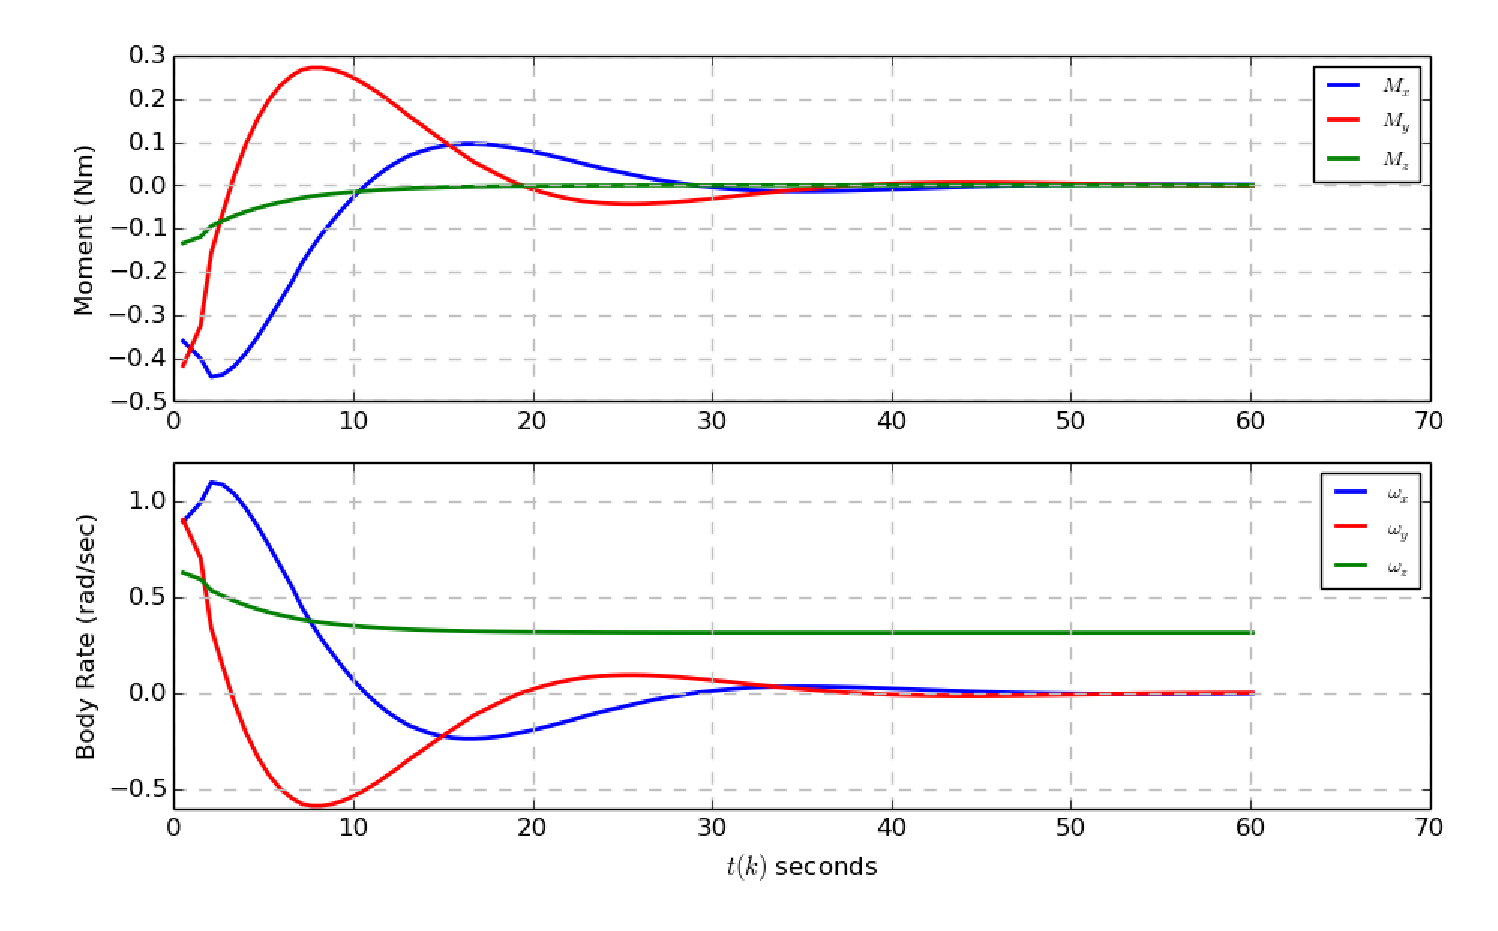
\psfig{file=figures/p_rate_control.eps,width=6in}}
  \caption{P rate control}
  \label{fig:PRateControl}
\end{figure}

\subsection{PID Rate Controller}
\label{subsec:PIDRateControl}

Expanding the proportional controller to include the integral and derivative term as shown in Equation \ref{eqn:PIDRateControl} can improve the performance slightly in the perfect measurement tests, but more importantly provides tools for dealing with noisy measurements when assessing observer-based controllers in Chapter \ref{chap:ObserverBasedControls}.  The integral and derivative terms are implemented with the $\Delta t_k$ adaptive step as with the PID estimator to help account for inconsistencies in update intervals by tracking the step size at each update.
\begin{equation}
  \begin{aligned}
    \bs{M}_{\omega} &= \bs{K}_{\omega p} \bs{\omega}_e + \bs{K}_{\omega i} \cdot (\Delta t_k \bs{I})\cdot \bs{\omega}_e + \bs{K}_{\omega d} \cdot \left(\frac{1}{\Delta t_k} \bs{I}\right) \cdot \bs{\omega}_e
  \end{aligned}
  \label{eqn:PIDRateControl}
\end{equation}
\begin{figure}[H]
  \centerline{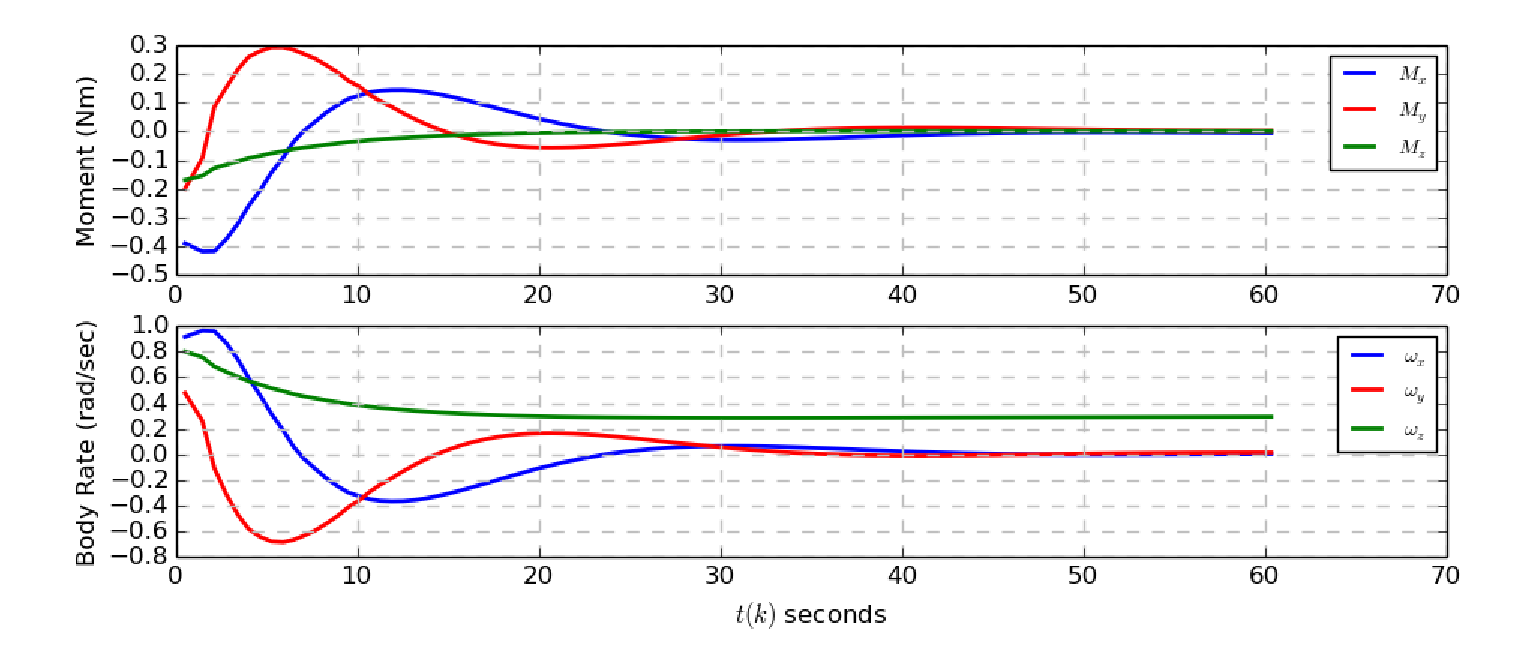
\psfig{file=figures/pid_rate_control.eps,width=6in}}
  \caption{PID rate control}
  \label{fig:PIDRateControl}
\end{figure}
The response curve in Figure \ref{fig:PIDRateControl} is generated from a random initial condition, and with the PID gains (Equation \ref{eqn:PIDRateControlGains}) tuned through gradient descent iterations based on minimizing the total control effort.  In the case of the perfect measurements, the addition correction two control terms generally reduce the overshoot of the response, but do not significantly shorten the time to bring the system to a steady state.
\begin{equation}
  \begin{aligned}
    \bs{K}_{\omega p} &= \begin{bmatrix} 0.424 & 0 & 0 \\ 0 & 0.416 & 0 \\ 0 & 0 & 0.346 \end{bmatrix},
    \bs{K}_{\omega i} = \begin{bmatrix} 0.006 & 0 & 0 \\ 0 & 0.003 & 0 \\ 0 & 0 & 0.005 \end{bmatrix} \\
    \bs{K}_{\omega d} &= \begin{bmatrix} 0.044 & 0 & 0 \\ 0 & 0.072 & 0 \\ 0 & 0 & 0.042 \end{bmatrix}
  \end{aligned}
  \label{eqn:PIDRateControlGains}
\end{equation}
Figure \ref{fig:PIDRateControlMoments} shows how the moments from each of the PID components contributes to the overall moments applied.  The addition of the derivative term gives the system a slightly quicker response that just the P-controller, and in this perfect measurement scenario the the overall performance of the system would benefit from the integral term being removed altogether since it doesn't contribute much to the initial response and even causes a larger steady state error than the P-controller.
\begin{figure}[H]
  \centerline{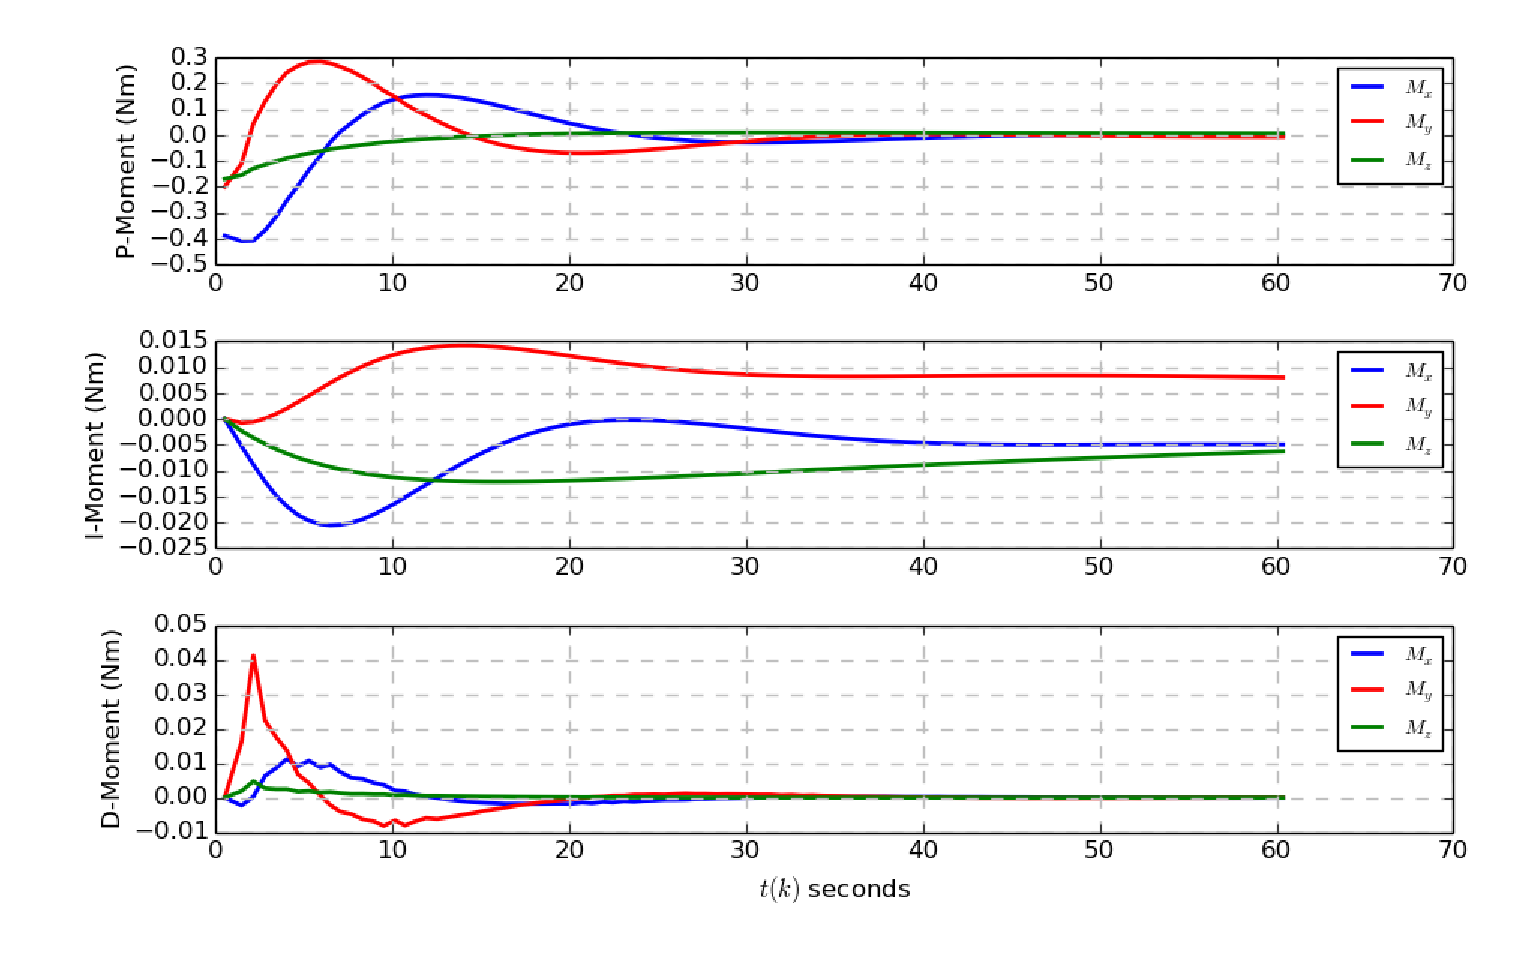
\psfig{file=figures/pid_rate_control_moments.eps,width=6in}}
  \caption{PID rate control moments}
  \label{fig:PIDRateControlMoments}
\end{figure}

\subsection{Sliding Mode Controller}
\label{subsec:SlidingModeController}

The Sliding Mode Controller (SMC) operates similarly to a proportional controller and is governed by the equation
\begin{equation}
  \bs{M}_{\omega} = \bs{L}_{\omega} \bs{\omega}_e + \bs{K}_{\omega}\bs{1}_s \big(\bs{\omega}_e \big)
  \label{eqn:SMController}
\end{equation}
where $\bs{L}_{\omega}$ is the proportion gain and the $\bs{1}_s$ function can take a number of forms such as the signum and arctangent function.  In this thesis the smc uses the saturation function such that $\bs{1}_s$ is
\begin{equation}
  \bs{1}_s \big(\bs{\omega}_e \big) = sat \begin{bmatrix} \omega_{ex} / S_{\omega} &0 &0 \\ 0 & \omega_{ey} / S_{\omega} & 0 \\ 0 & 0 & \omega_{ez} / S_{\omega} \end{bmatrix}
\end{equation}
The response to the test configuration is very similar to that of the proportional controller as shown if Figure \ref{fig:SMCRateControl}.  Breaking the overall moment values into the separate term's contributions show in Figure \ref{fig:SMCRateControlMoments} shows the similar profile between the proportional and saturation term contributions with the exception of the peaks missing from the saturation response.  This behavior indicates a tendency for the SMC to gently pull the estimated system state toward the desired state if there is a large discrepancy, but as the two converge the strength of the corrections increases causing the two state to stick more tightly together.
\begin{figure}[H]
  \centerline{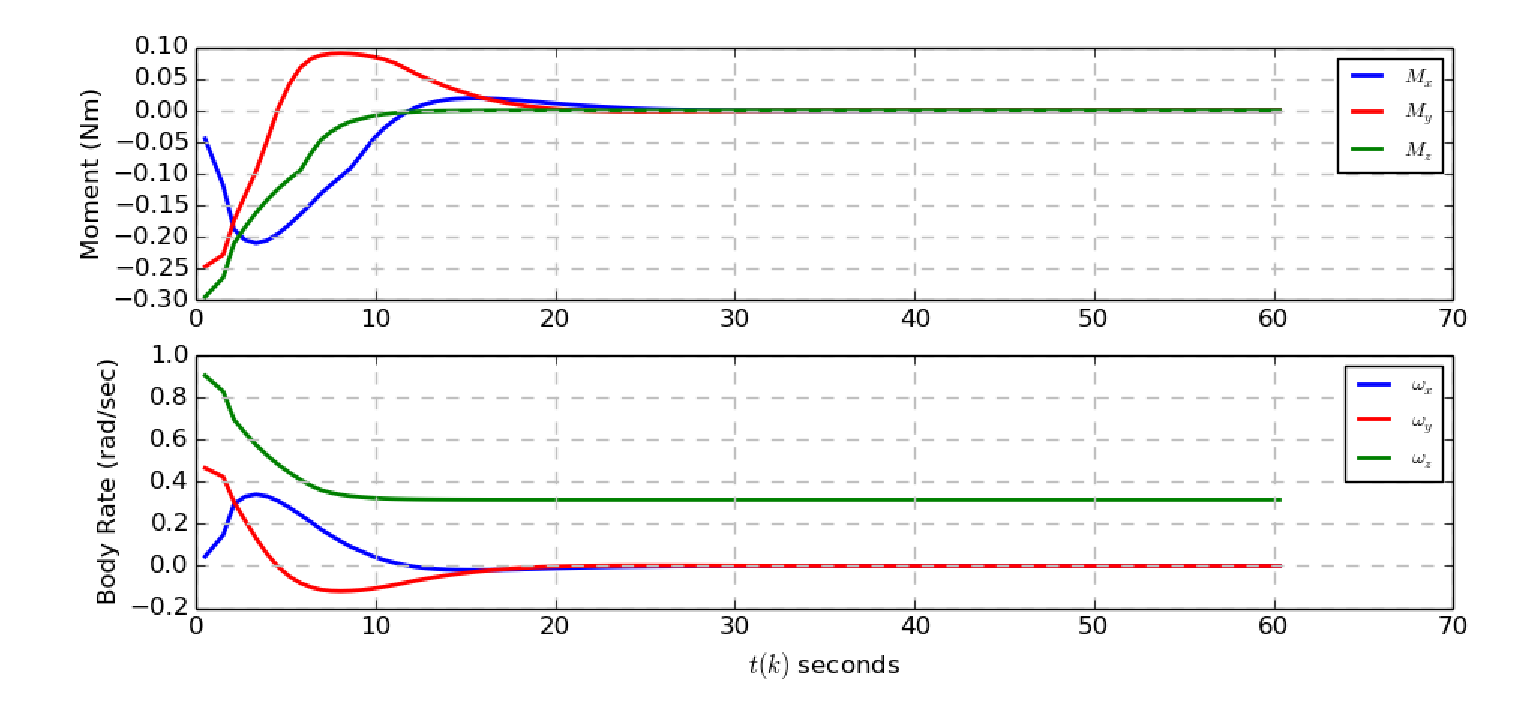
\psfig{file=figures/smc_rate_control.eps,width=6in}}
  \caption{SMC rate control}
  \label{fig:SMCRateControl}
\end{figure}
\begin{figure}[H]
  \centerline{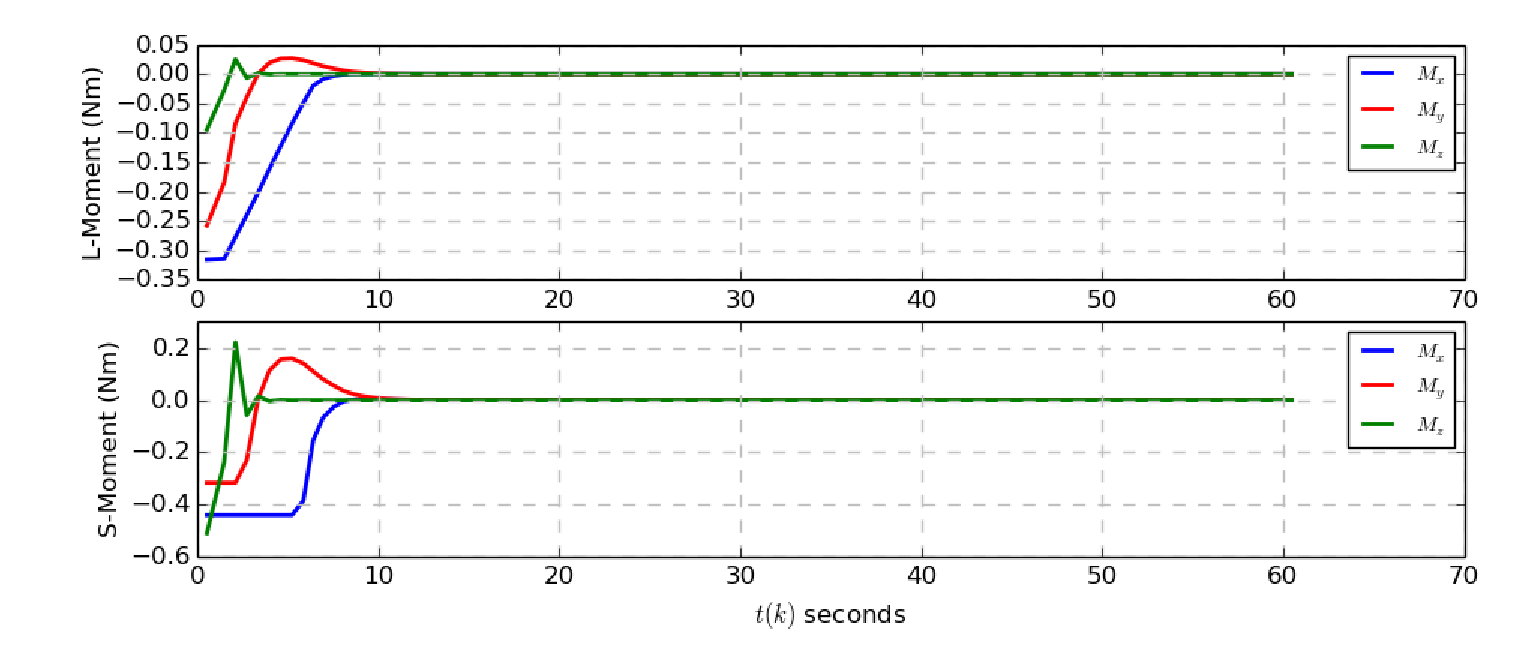
\psfig{file=figures/smc_rate_control_moments.eps,width=6in}}
  \caption{SMC rate control moments}
  \label{fig:SMCRateControlMoments}
\end{figure}
The SMC response in Figures \ref{fig:SMCRateControl} and \ref{fig:SMCRateControlMoments}, is generated with the following gain values tuned through a gradient descent algorithm.
\begin{equation}
    \bs{L}_{\omega} = \begin{bmatrix} 0.5264 & 0 & 0 \\ 0 & 0.3848 & 0 \\ 0 & 0 & 0.5976 \end{bmatrix},
    \bs{K}_{\omega} = \begin{bmatrix} 0.4724 & 0 & 0 \\ 0 & 0.4542 & 0 \\ 0 & 0 & 0.4049 \end{bmatrix},
    S_{\omega} = 0.0940
  \label{SMCRateControlGains}
\end{equation}

\section{Nutation Correction}
\label{sec:NutationCorrection}

Section \ref{subsec:PIDRateControl} covered the design of the rate controller which addresses the first goal of the controller to maintain a spin rate of $\omega_z = 3$ rpm.  This section focuses on the nutation control problem that to simplicity the overall controller design is decoupled from the rate control.  The combined control effort would be

\begin{equation}
    \bs{M}(t_{k+1}) = \bs{M}_{q}(t_{k+1}) + \bs{M}_{\omega}(t_{k+1})
\end{equation}

The nutation control focuses or the differences between the estimated quaternion attitude and the desired quaternion attitude.  The addition of the desired body rates of $\omega_x = \omega_y = 0$ can be added later if needed.  Since the work in Section \ref{chap:StateError} shows that working with the radian measure of the rotational quaternion had significant benefits over the traditional full state difference method, a similar approach is used for the nutation control.

\subsection{P Attitude Control}
\label{subsec:PAttitudeControl}

Starting with a simplest design of the proportional attitude control where the error quaternion $\bs{q}_e$ is defined in terms of the estimated quaternion $\bs{\hat{q}}$ and the desired quaternion attitude $\bs{q}_d$ as

\begin{equation}
  \bs{q}_e = \bs{\hat{q}}^* \otimes \bs{q}_d
\end{equation}

To generate the moments needed to correct for the error in attitude, the P controller can take advantage of the quaternion notation where the vector portion identifies the Euler axis, and whose components can be used as the basis for the correction moment by scaling them by the radian angular measurement of the error and a proportional gain.

\begin{subequations}
  \begin{align}
    \bs{M}_{q} &= \left[-2 K_{qp} \cos^{-1} \big(\hat{q}_{e0} \big) \right] \bs{\hat{e}}_e \\
    \text{where } \bs{\hat{e}}_e &= \frac{\bs{\hat{v}}_e}{|\bs{\hat{v}}_e|}
  \end{align}
  \label{eqn:PAttitudeControl}
\end{subequations}

To assess the basic functionality of the proportional quaternion in Equation \ref{eqn:PAttitudeControl}, the controller is run with $K_{qp} = 0.01$ and told to return the quaternion to the standard state with the body's reference frame aligned with the global reference frame.  The TableSat is given an initial condition of

\begin{equation}
  \bs{x}_0 = \begin{bmatrix} 0 \bs{i} -0.0477 \bs{j} -0.477 \bs{k} +0.8778 \\ 0 \bs{i} -0.01 \bs{j} 0.2 \bs{k} \end{bmatrix}
\end{equation}


\begin{figure}[H]
  \centerline{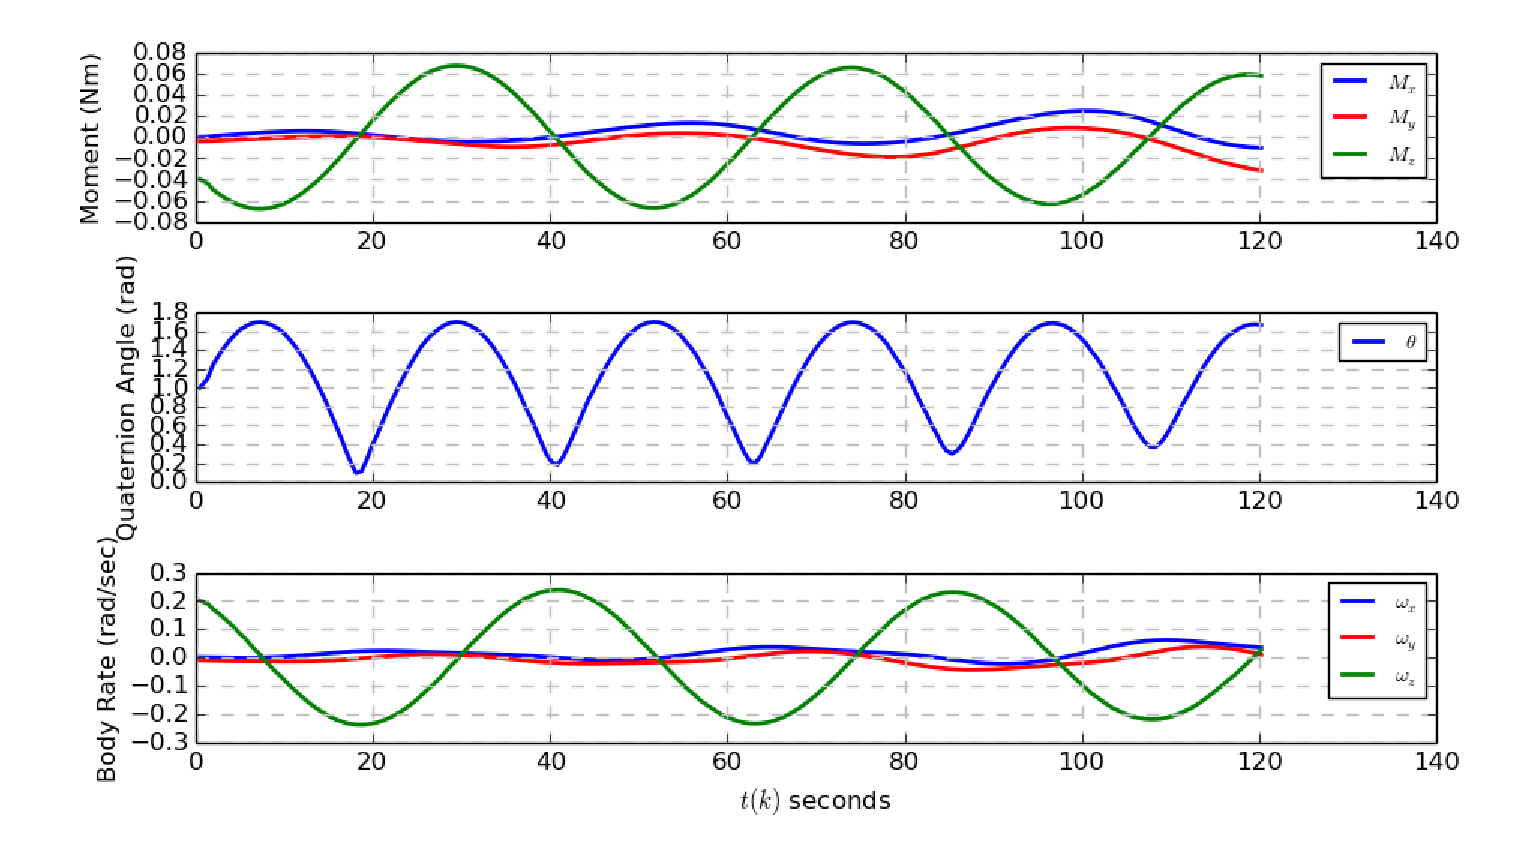
\psfig{file=figures/p_attitude_control.eps,width=6in}}
  \caption{P Attitude Control}
  \label{fig:PAttitudeControl}
\end{figure}

The results shown in \ref{fig:PAttitudeControl} are very promising.  The full three degree of freedom (DOF) object with an initial out of plane offset and initial body rates is able to oscillate about the desired set point with the use of a single gain being combined with the components of the current step's quaternion attitude.

Combining the proportional attitude control in Equation \ref{eqn:PAttitudeControl} with the proportional body rate control in Equation \ref{eqn:PRateControl} gives

\begin{subequations}
  \begin{align}
    \bs{M}(t_{k+1}) &= \left[-2 K_{qp} \cos^{-1} \big(\hat{q}_{e0}(t_{k+1}) \big) \right] \bs{\hat{e}}_e(t_{k+1}) + \bs{K}_{\omega p} \bs{\omega}_e(t_{k+1})\\
    \text{where } \bs{\hat{e}}_e(t_{k+1}) &= \frac{\bs{\hat{v}}_e(t_{k+1})}{|\bs{\hat{v}}_e(t_{k+1})|} \\
    \bs{\omega}_e(t_{k+1}) &= \bs{\omega}_d - \bs{\hat{\omega}}(t_{k+1})
  \end{align}
  \label{eqn:PAttitudeAndRateControl}
\end{subequations}

After an iterative gradient descent to minimize the control effort, the following gains provided the best performance against a variety of initial conditions.

\begin{equation}
  K_{qp} = 0.0912, \bs{K}_{\omega p} = \begin{bmatrix} 0.494 & 0 & 0 \\ 0 & 0.583 & 0 \\ 0 & 0 & 0.624 \end{bmatrix}
\end{equation}

Figure \ref{fig:PAttitudeRateControl} shows the system's response when bringing a system into the standard orientation from an initial condition of

\begin{equation}
  \bs{x}_0 = \begin{bmatrix} -0.202 \bs{i} -0.0581 \bs{j} -0.222 \bs{k} +0.952 \\ 0.585 \bs{i} +0.0919 \bs{j} +0.999 \bs{k} \end{bmatrix}
\end{equation}

\begin{figure}[H]
  \centerline{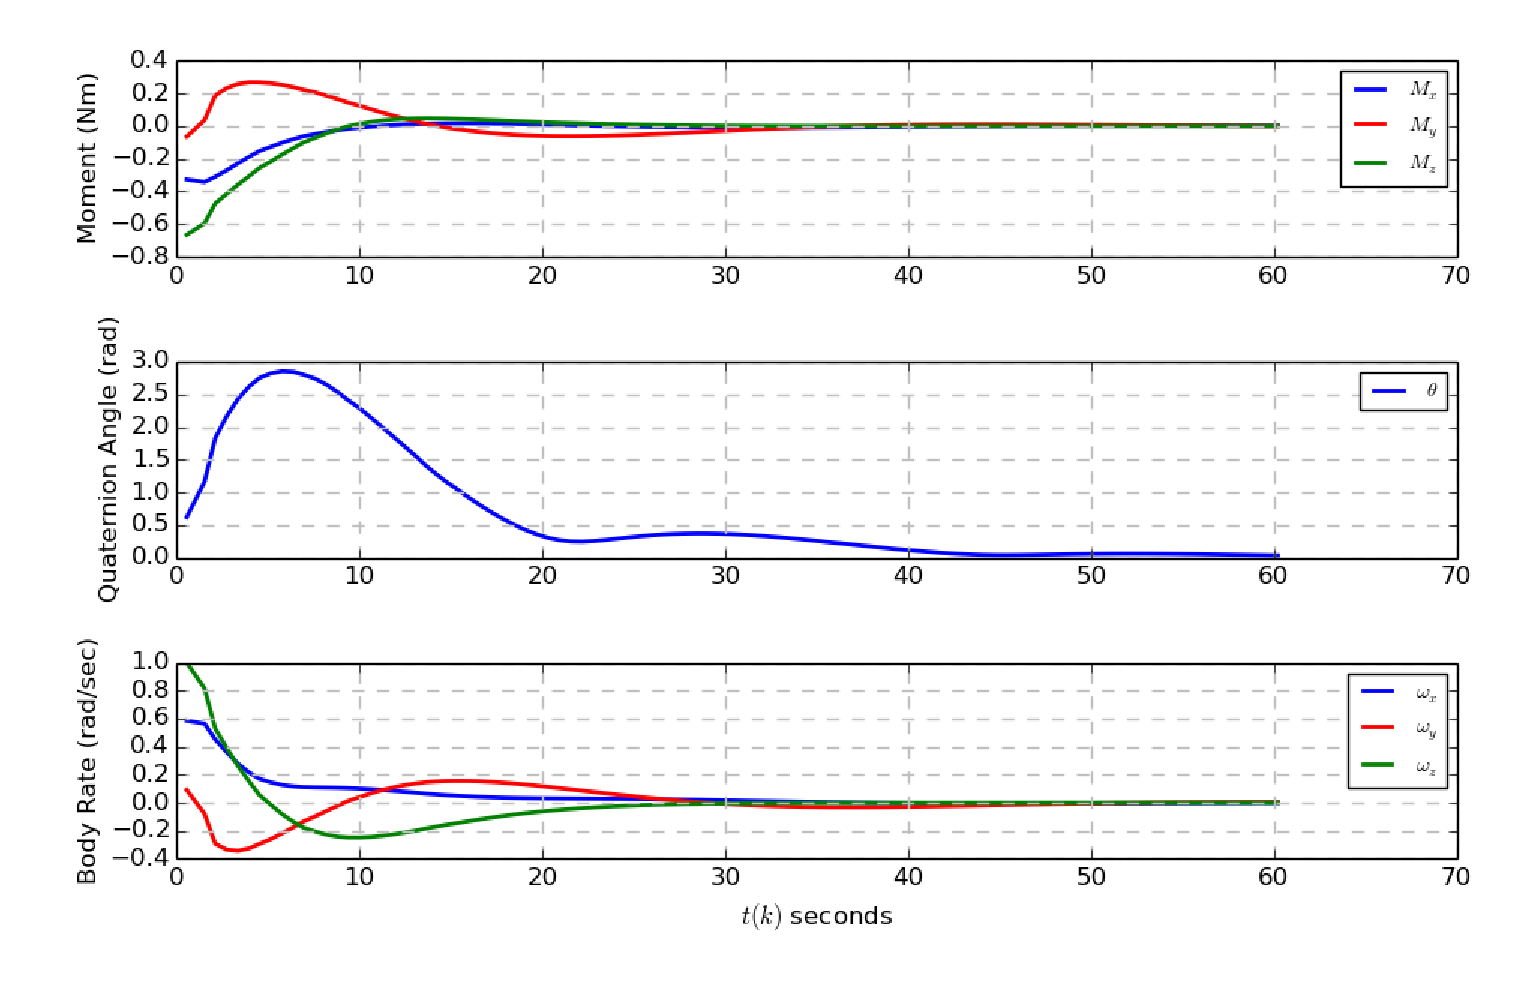
\psfig{file=figures/p_attitude_and_rate_control.eps,width=6in}}
  \caption{P Attitude and Rate Control}
  \label{fig:PAttitudeRateControl}
\end{figure}

Another random initial condition test run under the same parameters, provides additional support for the choice of the multiplicative quaternion corrections and error quaternions.  With the system initialed to the state

\begin{equation}
  \bs{x}_0 = \begin{bmatrix} -0.0134 \bs{i} -0.0611 \bs{j} -0.0347 \bs{k} +0.997 \\ 0.259 \bs{i} +0.899 \bs{j} +0.402 \bs{k} \end{bmatrix}
\end{equation}

The response in Figure \ref{fig:PAttitudeRateControlWithAntipodalRollOver} shows that at about five seconds into the control run, the control effort moments jump.  This can happen when the system passes close to a point antipodal from the desired orientation.  The proportional rate controller is slowing down the initial body rates while the quaternion proportional controller is attempting to unwind the angle to bring the system back to the desired orientation.  At about five seconds into the test run, the rate controller has reduced much of the initial spin rate.  At that same time the attitude quaternion angle shows it is passing a point that requires a 3.14 radian turn to bring it back to the desired orientation.  At this point it is more efficient to allow the rotation around the rest of the rotation and ease it into the desired state rather that bringing the system to a halt and unwinding the whole way.  This behavior in advantageous, but the additional benefit of using the quaternion multiplicative correction is that it is built into the rotational quaternion that 0 and $2\pi$ are the same orientation.  So even though the desired orientation is a zero degree angle as is performed in Figure \ref{fig:PAttitudeRateControl}, this test converges the system to the more efficient $2\pi$ orientation as shown in the center graph in Figure \ref{fig:PAttitudeRateControlWithAntipodalRollOver}.

\begin{figure}[H]
  \centerline{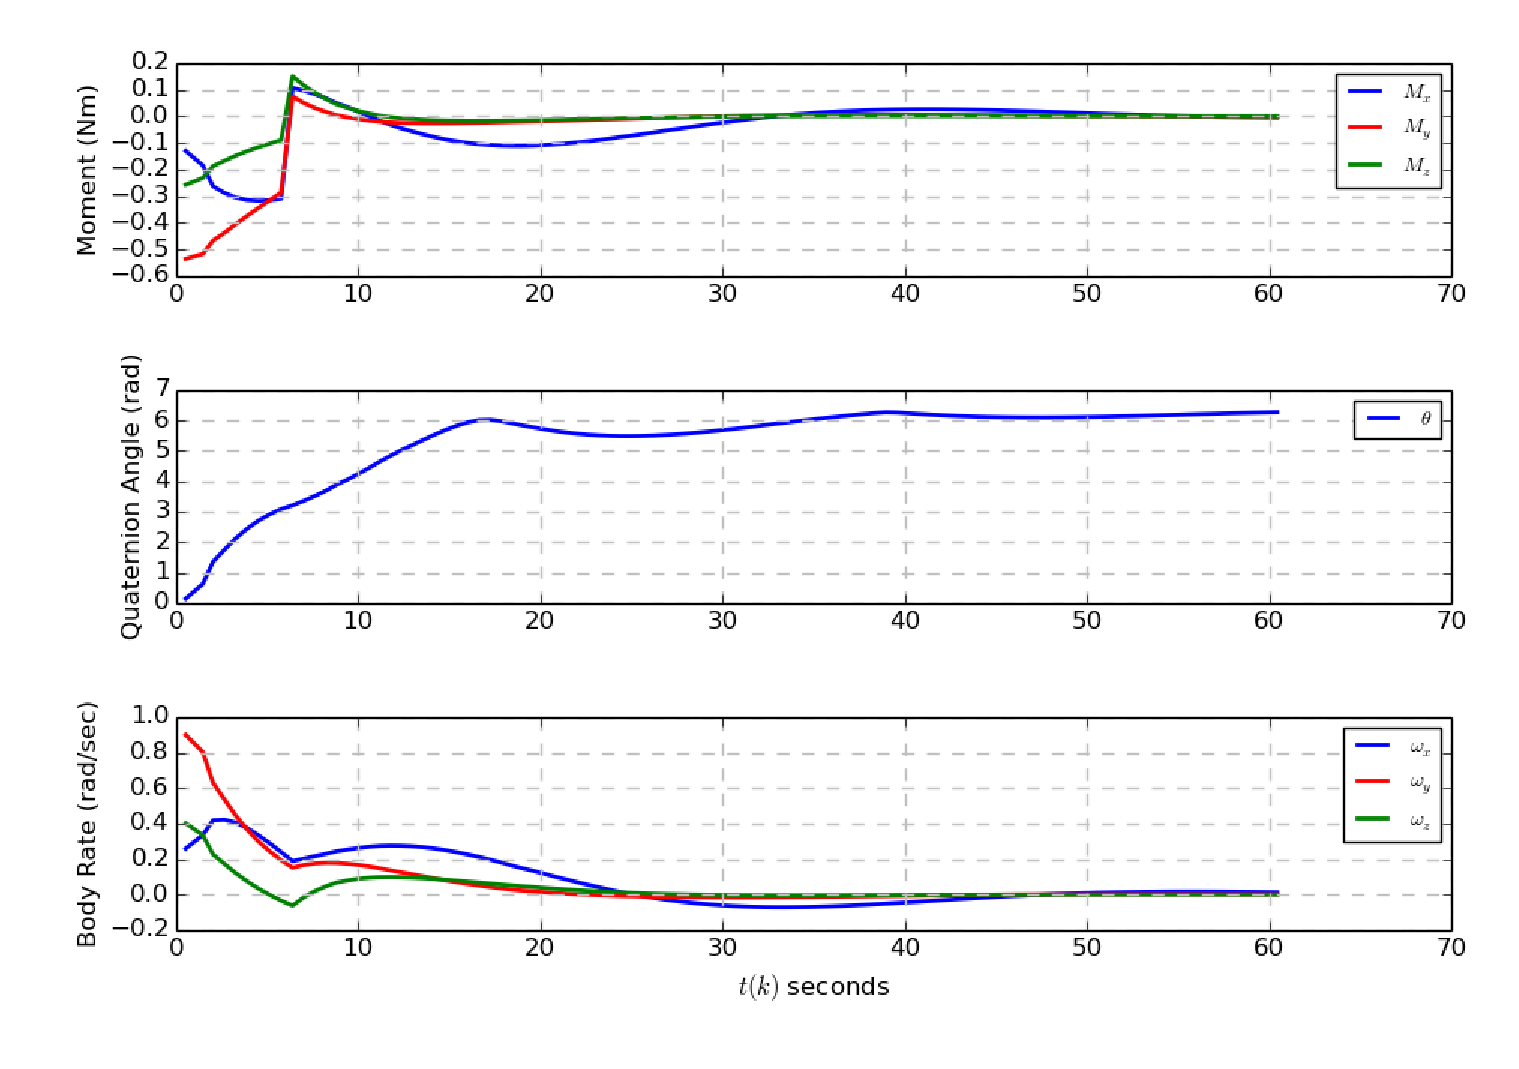
\psfig{file=figures/p_attitude_and_rate_control_with_180_roll_over.eps,width=6in}}
  \caption{P Attitude and Rate Control with Antipodal Roll Over}
  \label{fig:PAttitudeRateControlWithAntipodalRollOver}
\end{figure}

This proportional attitude controller has shown to work extremely well at correcting for a variety of conditions, but unlike the needs of the NASA MMS mission, it's target attitude is the standard orientation of body rates aligned with the global reference frame and with no body rates.  The following sections attempt to isolate and correct for a nutation outside of the spin plane independent of the rotation about the $z$-axis.

\subsection{Quaternion Decomposition}
\label{subsec:QuaternionDecomposition}

In order to proceed with isolating and correcting for nutation out side of the global $xy$ spin plane, a method for quantifying the nutation from the quaternion attitude is required.  From Equation \ref{eqn:RotationalQuaternionDefinition}, the definition of the rotational quaternion shows that if the system is in a non-nutated state the $q_1$ and $q_2$ components must be zero.

\begin{equation}
  \bs{q}_dn = 0 \bs{i} + 0 \bs{j} +q_3 \bs{k} + q_0
  \label{eqn:NutationDesiredQuaternion}
\end{equation}

Since the state quaternion represents a single rotation about the Euler axis and a rotational quaternion can be composed from multiple quaternions through a quaternion multiplication (Section \ref{subsubsec:QuaternionMultiplication}), the attitude quaternion could be created from a rotation about the $z$ axis and a nutation.  The rotation $\bs{q}_r$ and nutation $\bs{q}_n$ quaternion are defined as

\begin{subequations}
  \begin{align}
    \bs{q}_r &= 0 \bs{i} + 0 \bs{j} + r_3 \bs{k} + r_0\\
    \bs{q}_n &= -n_1 \bs{i} - n_2 \bs{j} + 0 \bs{k} - n_0 \\
    \text{where: } n_1 &= Q \cdot n_2 \\
    n_2 &= \sqrt{\frac{1 - n_0^2}{Q^2 + 1}} \\
    Q &= \frac{q_0 q_1 - q_2 q_3}{q_0 q_2 + q_1 q_3} \\
    r_3 &= q_3 / n_0 \\
    r_0 &= q_0 / n_0 \\
    n_0 &= \sqrt{q_0^2 + q_3^2}
  \end{align}
  \label{eqn:DecomposeQuaternion}
\end{subequations}

This thesis refers to the method decomposition of a quaternion through the method in equation \ref{eqn:DecomposeQuaternion} as


Equation \ref{eqn:DecomposeQuaternion} has been built into the TSatPy library for use in the controller.  The code snippet below demonstrates the decompose method at work.  Lines 3-4 define a known rotation and nutation.  At line 8 the normal multiplication operation has been converted to a quaternion multiplication to combine quaternions into a single attitude quaternion that may be encountered in a simulation or experimental test.  Recall from Section \ref{subsec:QuaternionAttitude} that the quaternion multiplication is not commutative, so this combination represents a rotation first then a nutation.  At line 11, the single quaternion representation is asked to break itself into a rotation and nutation quaternion according as defined in Equation \ref{eqn:DecomposeQuaternion}.  The resulting decomposition can been seen in lines 16-22 to match the chosen rotation and nutation.

\begin{singlespace}
  \begin{minted}[mathescape,linenos,numbersep=10pt,frame=lines,framesep=2mm]{python}
from TSatPy.State import Quaternion

q_r1 = Quaternion([0,0,1], radians=1.2)
q_n1 = Quaternion([1,-1,0], radians=-0.2)
print("q_r1: %s" % (q_r1))
print("q_n1: %s" % (q_n1))

q = q_n1 * q_r1
print("q:    %s" % (q))

q_r2, q_n2 = q.decompose()
print("q_r2: %s" % q_r2)
print("q_r2: %s" % q_n2)

# Prints Out
# q_r1: <Quaternion [-0 -0 -0.564642], 0.825336>
# q_n1: <Quaternion [0.0705929 -0.0705929 0], 0.995004>

# q:    <Quaternion [0.0981226 -0.0184031 -0.561822], 0.821212>

# q_r2: <Quaternion [0 0 -0.564642], 0.825336>
# q_r2: <Quaternion [0.0705929 -0.0705929 -0], 0.995004>
  \end{minted}
\nocite{minted}
\end{singlespace}

Now that there is a defined method for separating the allowed rotation from the unwanted nutation, the next section incorporates it into a attitude controller.

\subsection{Quaternion to Moment Conversion}

\TODO{this}
\begin{equation}
  \bs{M}_{q} = \left[-2 K_{qp} \cos^{-1} (q_{0n}) \right] \bs{\hat{e}}_n
  \label{eqn:QuaternionToMomentConversion}
\end{equation}


\subsection{P Nutation Control}
\label{subsec:PNutationControl}

Since the previous section's P-controller proved very successful at attitude control, this section attempts to loosen the restrictions on the desired attitude to allow for free rotation about the global reference frame's $z$-axis while correcting for nutation out of the spin plane making use of the quaternion decomposition in Equation \ref{eqn:DecomposeQuaternion}.

In this test, a random attitude is chosen and the controller's task is to bring the satellite level regardless of the point in the rotation about the $z$-axis.  From Equation \ref{eqn:PAttitudeControl},    As with previous test runs, parameters were tuned to obtain a minimum control effort.

\begin{equation}
  \bs{M}_{q} = \left[-2 K_{qp} \cos^{-1} (q_{0n}) \right] \bs{\hat{e}}_n
  \label{eqn:PNutationControl}
\end{equation}


The test is initialized at rest at an orientation of a 1.26 radian rotation about $-0.25 \bs{i} -0.406\bs{j} -0.879\bs{k}$.  With a proportional gain $K_{qp} = 0.152$, the P-controller behaved as a normal by oscillating back and forth about the desired orientation.  What is notable though is that even though the system is in a state rotated away from the standard orientation, the $M_z$ term remains 0 since the controller only uses the nutation portion of the quaternion state.

\begin{figure}[H]
  \centerline{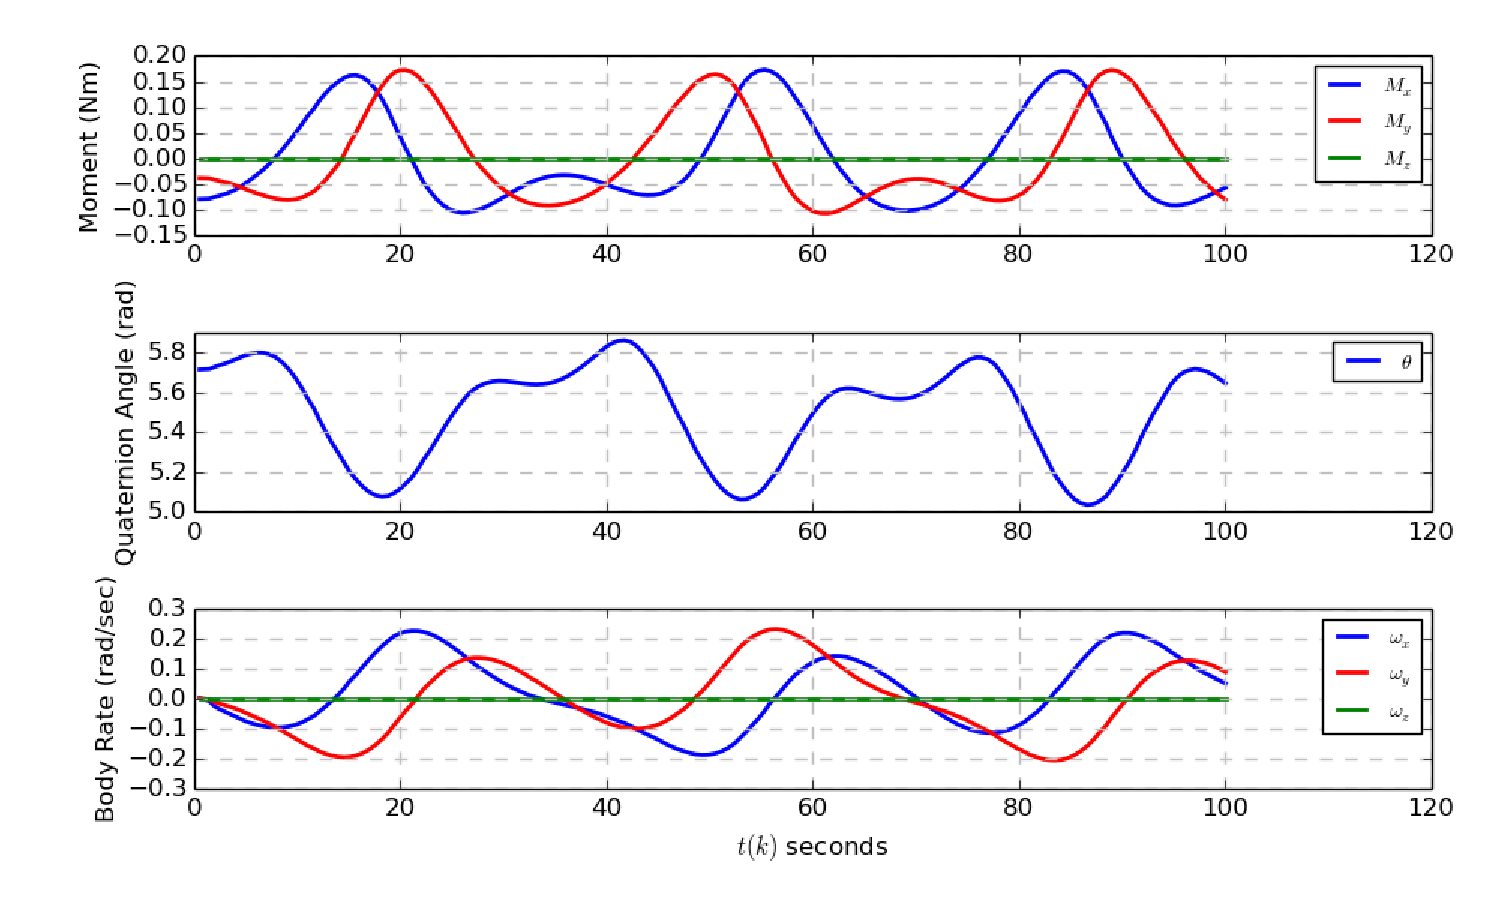
\psfig{file=figures/p_nutation_control.eps,width=6in}}
  \caption{P Nutation Control}
  \label{fig:PNutationControl}
\end{figure}

While this controller is correctly pushing the state to the spin plane there is no mechanism to damp out the oscillations.

\subsection{P Rate and Nutation Control Starting at Rest}
\label{subsec:PRateNutationControlStartingatRest}

Since the proportional attitude control converged to the desired state through the addition of a proportional body rate controller, this section adds a body rate controller to the P-Nutation controller from the previous section.  Figure \ref{fig:PNutationRateControl} shows the result of a test with an initial conditions of $\bs{q}_0 = -0.289\bs{i} -0.0130 \bs{j} -0.154 \bs{k} + 0.945$ and body rates $\omega_x = \omega_f = \omega_z = 0$.  The proportional nutation and body rate controllers are run with the parameters

\begin{equation}
  K_{qp} = 0.268, \bs{K}_{\omega p} = \begin{bmatrix} 0.414 & 0 & 0 \\ 0 & 0.559 & 0 \\ 0 & 0 & 0.418 \end{bmatrix}
\end{equation}

\begin{figure}[H]
  \centerline{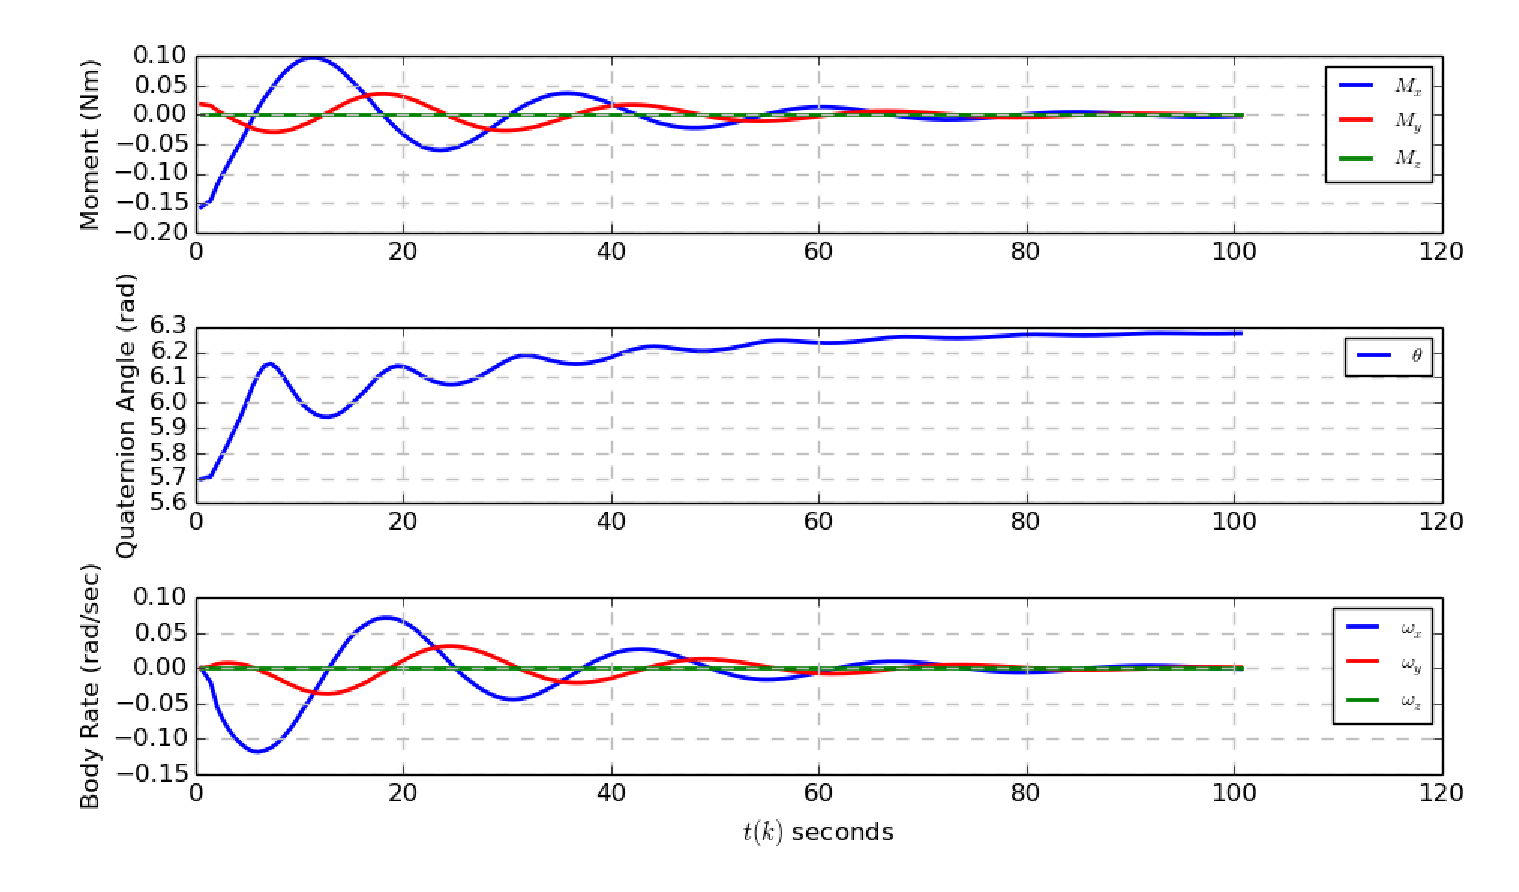
\psfig{file=figures/p_nutation_and_rate_control.eps,width=6in}}
  \caption{P Nutation and Rate Control}
  \label{fig:PNutationRateControl}
\end{figure}

\subsection{PID Rate and Nutation Control Using Quaternion Decomposition}
\label{subsec:PIDRateandNutationControl}
In a full state control configuration the plant is initialized to a random attitude and body rate of
\begin{equation}
  \bs{x}_{ic} = \begin{bmatrix} -0.102 \bs{i} -0.478 \bs{j}-0.0678 \bs{k} + 0.870 \\ 0.710 \bs{i} + 0.155 \bs{j} + 0.377 \bs{k} \end{bmatrix}
\end{equation}
unlike with the previous simulations in this chapter this run is configured to control both the attitude and body rate.  The controller is set with the desired state of
\begin{equation}
  \bs{x}_d = \begin{bmatrix} 0 \bs{i} +0 \bs{j} +0 \bs{k} + 1 \\ 0 \bs{i} + 0 \bs{j} + 0.314 \bs{k} \end{bmatrix}
\end{equation}
The attitude quaternion and body rate desired states are at odds with each other.  The identity quaternion sets the desired attitude to be fixed with the body-fixed reference frame aligned with the global reference frame.  The desired state defined by the body rate is to maintain a constant 0.314 rad/sec rotation about the body $z$-axis, so it must both stay still and move at a constant pace.

Resolving this conflict takes advantage of the quaternion decomposition derived in Equation \ref{eqn:quaternion_decomposition_derivation} and applies it to the estimated state's quaternion.  In effect, removing any rotational information from the quaternion leaving nutation and body rate data to feed into the controller.  The initial state from the estimator is
\begin{equation}
  \bs{\hat{x}}(t_{k}) = \begin{bmatrix} \bs{\hat{q}}(t_{k}) \\ \bs{\hat{\omega}}(t_{k}) \end{bmatrix} = \begin{bmatrix} \bs{\hat{q}}_n(t_{k}) \otimes \bs{\hat{q}}_r(t_{k}) \\ \bs{\hat{\omega}}(t_{k}) \end{bmatrix}
\end{equation}
and dropping the rotational component gives the modified state estimation as
\begin{equation}
  \bs{\hat{x}}^+(t_{k}) = \begin{bmatrix} \bs{\hat{q}}_n(t_{k})  \\ \bs{\hat{\omega}}(t_{k}) \end{bmatrix}
\end{equation}
The controller's state error is then calculated as
\begin{equation}
  \bs{x}_e(t_{k}) = \begin{bmatrix} \bs{q}_e(t_{k}) \\ \bs{\omega}_e(t_{k}) \end{bmatrix} = \begin{bmatrix} \bs{q}_d^*(t_{k}) \otimes \bs{\hat{q}}_n(t_{k}) \\ \bs{\hat{\omega}}(t_{k}) - \bs{\omega}(t_{k}) \end{bmatrix}
\end{equation}
Similar to the PID estimator in Equation \ref{eqn:PIDEstimatorwithPredictionUnforcedMotion}, the moments calculated by the controller is a summation of the quaternion based correction and the body rate correction moments
\begin{equation}
  \bs{M} = \bs{M}_q + \bs{M}_{\omega}
\end{equation}

Taking the integral $\bs{q}_{ei}$ and derivative $\bs{q}_{ed}$ quaternions from Equations \ref{eqn:IEstimator} and \ref{eqn:DEstimator} and the conversion from quaternion to moments in Equation \ref{eqn:QuaternionToMomentConversion}.  The quaternion portion of the moment correction is
\begin{equation}
  \bs{M}_{q} = \left[-2 K_{qp} \cos^{-1} (q_{0e}) \right] \bs{\hat{e}}_e + \left[-2 K_{q} \cos^{-1} (q_{0ei}) \right] \bs{\hat{e}}_{ei} + \left[-2 K_{q} \cos^{-1} (q_{0ed}) \right] \bs{\hat{e}}_{ed}
\end{equation}
where $\bs{\hat{e}}_e, \bs{\hat{e}}_{ei}, \bs{\hat{e}}_{ed}$ are the Euler axes for the quaternion error, quaternion error integral, and quaternion error derivative respectively.

The body rate portion of the moment correction is
\begin{equation}
  \bs{M}_{\omega} = \bs{K}_{\omega p} \cdot \bs{\omega}_e(t_{k}) + \bs{K}_{\omega i} \cdot (\Delta t_k \bs{I})\cdot \bs{\omega}_e(t_{k}) + \bs{K}_{\omega d} \cdot \left(\frac{1}{\Delta t_k} \bs{I}\right) \cdot \bs{\omega}_e(t_{k})
\end{equation}



with quaternion error to moment gains of
\begin{equation}
  K_{pq} = 0.11112, K_{iq} = 0.00925, K_{dq} = 0.23122
\end{equation}
and body rate error to moment gains of
\begin{equation}
  \begin{aligned}
  \bs{K}_{\omega p} &= \begin{bmatrix} 0.56073&0&0 \\ 0&0.46617&0 \\ 0&0&0.62449 \end{bmatrix} \\
  \bs{K}_{\omega i} &= \begin{bmatrix} 0.59005&0&0 \\ 0&0.46463&0 \\ 0&0&0.42009 \end{bmatrix} \\
  \bs{K}_{\omega d} &= \begin{bmatrix} 0.34528&0&0 \\ 0&0.56419&0 \\ 0&0&0.54984 \end{bmatrix} \\
  \end{aligned}
\end{equation}

% x_est_ic:    <Quaternion [-0.102078 -0.477679 -0.067834], 0.869943>, <BodyRate [0.70997 0.155469 0.377068]>
% (matrix([[-0.20699052],
%         [-0.968625  ],
%         [-0.13755192]]), 1.031418752494432)

    % kwargs = {'Kpq': 0.11111822352039165, 'Kpwy': 0.46617055725812362, 'Kiq': 0.0092460954947930132, 'Kiwy': 0.56418807555550599, 'Kpwx': 0.56072598825499542, 'Kiwx': 0.34527737331963193, 'Kpwz': 0.62449446448477242, 'Kiwz': 0.54983623166470164, 'Kdwx': 0.59004903787603236, 'Kdwy': 0.4646265536024109, 'Kdwz': 0.42009087143770402, 'Kdq': 0.23121875724788765}

% # Kpq:
% #   val: 0.111118 range: 0.02,0.22    std: 0.0340246
% # Kpwx:
% #   val: 0.560726 range: 0.39,0.71    std: 0.0474869
% # Kpwy:
% #   val: 0.466171 range: 0.17,0.65    std: 0.0840252
% # Kpwz:
% #   val: 0.624494 range: 0.32,0.84    std: 0.0970963
% # Kiq:
% #   val: 0.0092461    range: 0.003,0.039  std: 0.00281212
% # Kiwx:
% #   val: 0.345277 range: 0.23,0.51    std: 0.0553643
% # Kiwy:
% #   val: 0.564188 range: 0.28,0.88    std: 0.115591
% # Kiwz:
% #   val: 0.549836 range: 0.29,0.81    std: 0.0990584
% # Kdq:
% #   val: 0.231219 range: 0.05,0.61    std: 0.0793672
% # Kdwx:
% #   val: 0.590049 range: 0.32,0.8 std: 0.107061
% # Kdwy:
% #   val: 0.464627 range: 0.12,0.72    std: 0.0881444
% # Kdwz:
% #   val: 0.420091 range: 0.27,0.63    std: 0.06911



\begin{figure}[H]
  \centerline{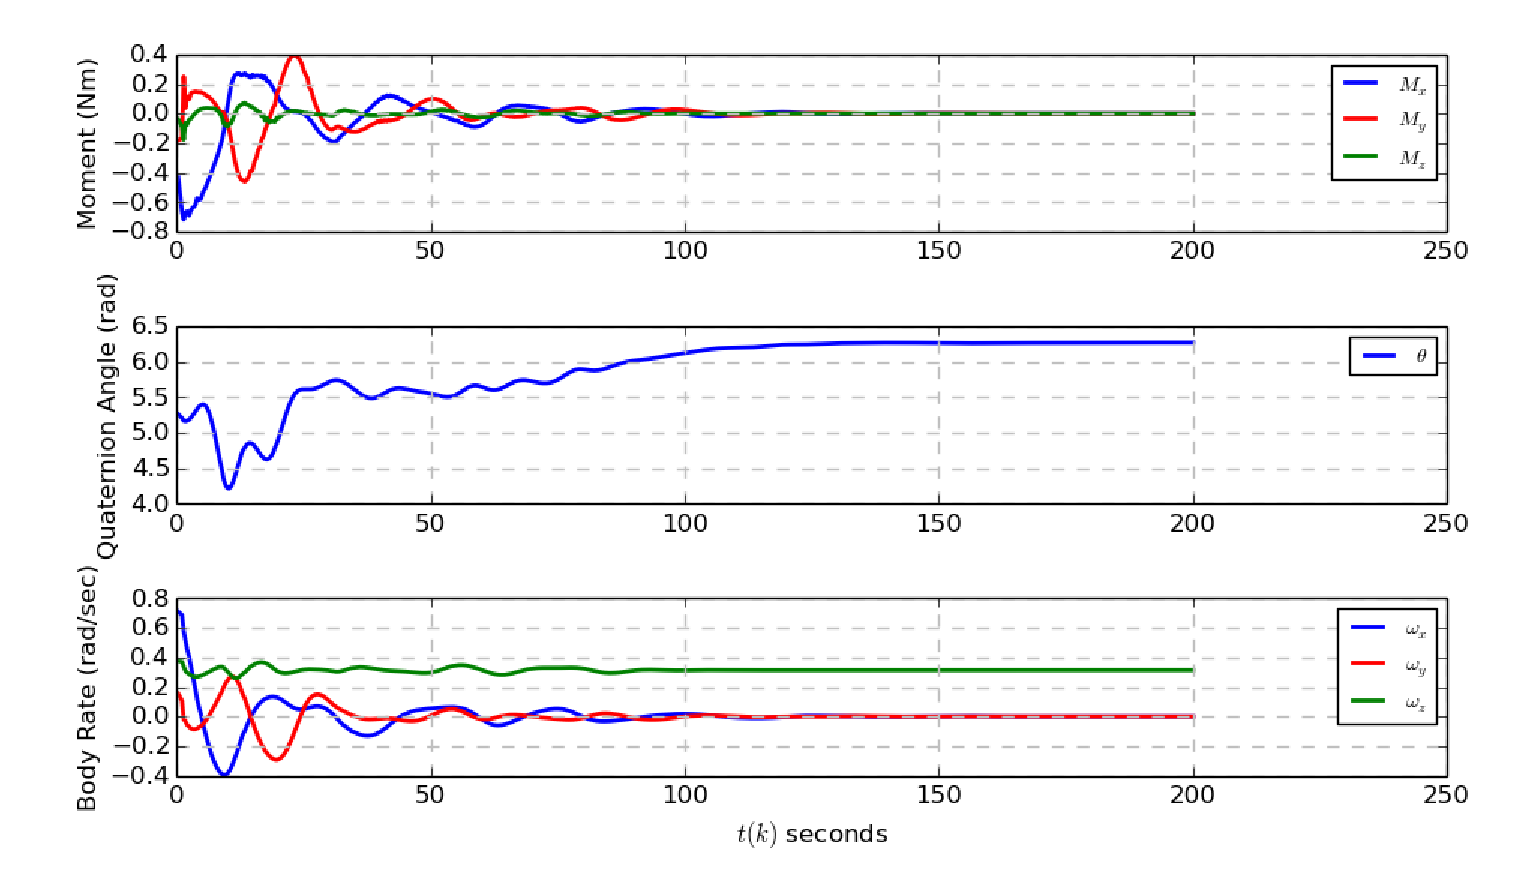
\psfig{file=figures/pid_attitude_and_rate_control.eps,width=6in}}
  \caption{PID Rate and Nutation Control}
  \label{fig:PIDNutationRateControl}
\end{figure}

\subsection{SMC Rate and Nutation Control}
\label{subsec:SMC}

\TODO{this}

\section{Comparative Analysis of PID and SMC Rate and Nutation Control}
\label{sec:ComparativeAnalysisofPIDandSMCRateandNutationControl}

\TODO{this}
